\newcommand{\Cont}{\mathcal{C}}%
\section{Introduction}
In abstraction of dynamical systems, the knowledge of the sequence of inputs applied to the plant might sometimes be preferable than the knowledge of the full state.
%
%The transient states of the system make the control synthesis more complex in some situation (small environment, or noisy environment).
%More accurate models (second integrator with a small discretization of the state space) could be used with some drawbacks on the complexity and on the computation time.
Hereby we present an abstraction of a dynamical model (discrete or continuous time) obtained by extending the state with the knowledge of the finite time input sequence lastly applied to the system.
We have successfully used this abstraction in order to control quadricopters. Abstraction obtained were a good alternative to solve the controller synthesis while keeping the complexity acceptable.


% Property that needs to be verified by the abstraction
Controller synthesis methods based on abstraction aim at finding an abstraction of a system. If a property verified by the abstraction is a sufficient condition for the system to verify the property, then it is possible to use controller synthesis methods. Such a relation is the alternating simulation relationship.


\section{Related work}
Talk about formal verifications methods.

The needs of discrete abstraction.


\section{Preliminaries}
%% MOVE THIS PART
In \cite{tabuada2009verification}, the link between in hybrid systems is investigated. 
\begin{nameddef}{System}\label{def:system}
$S = (X,X_0,\U, \systransition{S}{}, Y,H)$
where:
\begin{itemize}[noitemsep,nolistsep]
\item $X$ is a set of states;
\item $X_0 \subset X$ a set of initial states;
\item $\U$ a set of inputs;
\item $\systransition{S}{} \subseteq X \times \U \times X$ a transition relation ;
\item $Y$ a set of outputs;
\item $H:X \rightarrow Y$ an output map.\popQED
\end{itemize}
\end{nameddef}

Such a definition of the system cover both discrete and continuous time case of dynamical systems. For the continuous time, the time is included as part of the set of inputs. Then a transition of the dynamical system from $\x$ to $\x' = \traj(t,\x,\u)$ will be written: $\x \systransition{S}{t,\u} \x'$. For the discrete case, a transition correspond to 1 timestep. The sets of states and of inputs does not have to verify any specific property, they can be infinite of finite sets.

Note: in the future we will use a second equivalent notations for the transition relation $\systransition{S}{\u}$ of a system $S$: $\Post{S}{\u}$  defined for $\x \in X$ and $\u \in \U$ by:
\begin{equation}
\Post{S}{\u}(\x) = \{ \x \in X \mid \exists \x' \in X, \x \systransition{S}{\u} \x' \}
\end{equation}

The alternating simulation relation between 2 systems is the link between discrete abstraction and the continuous representation of this system.
For comoditiy, the definition of alternative simulation is rewritten here (\cite{tabuada2009verification}):
\begin{nameddef}{Alternating simulation} \label{def_alt_sim}
Let $\sysA$ and $\sysB$ 2 systems with $Y_a=Y_b$, $\sysA$ is alternatingly simulated by $\sysB$ if there exists a relation $R \subseteq X_a \times X_b$ that verify:
\begin{enumerate}[noitemsep,nolistsep]
\item $\forall x_{a0} \in X_{a0}, \exists x_{b0} \in X_{b0}, (x_{a0},x_{b0}) \in R$
\item $\forall (x_a,x_b) \in R, H_a(x_a) = H_b(x_b)$
\item $\forall (x_a,x_b) \in R, \forall u_{a} \in \U_{a}, \exists u_{b} \in \U_{b}$\\
$\forall x_b' \in \Post{\sysB}{u_b}(x_b),\exists x_a' \in \Post{\sysA}{u_a}(x_a), (x_a',x_b') \in R$
\popQED
\end{enumerate}
\end{nameddef}
The alternating simulation relation between $\sysA$ and $\sysB$ is weaker than the bisimulation relation (that require the alternating simulation relation between $\sysA$ and $\sysB$ and between $\sysB$ and $\sysA$).

Lets denote the composition of systems by the operator $\times$.
If $\sysA$ alternatingly simulate by $\sysB$ for a controller $\Cont$ composable with $\sysA$ or $\sysB$, then $\sysA \times \Cont$ verify the same reachability properties than $\sysB \times \Cont$, and $\sysB \times \Cont$ verify the same safety properties than $\sysA \times \Cont$.


%% INPUT SEQUENCE REACHABLE SETS
In the next part we will focus on systems with inputs memory. The knowledge of unobserved variables will be replaced by the knowledge of an input sequence $\Pastuseq$.

For a system $S$, let $\Reach{S}{U} \subseteq X$ defined for a finite sequence $U \in \U^\star$ of $N \in \mathbb{N}$ control actions by:
\begin{equation}
\begin{split}
\x \in \Reach{S}{U}
\Leftrightarrow &
\exists \x_0 \in X_0,
\forall i<N, \exists \x_i \in X,\\
&\x_0 \systransition{S}{\u_0} \x_1
\systransition{S}{\u_1} \dots
\systransition{S}{\u_{N-1}} \x
\end{split}
\end{equation}
$\Reach{S}{U}$ correspond to all the reachable states with the sequence inputs $U$.

%% Define the reached states:
\renewcommand{\v}{\vect{v}}
\newcommand{\useq}{\v_{1-n},\dots,\v_{0}}
\begin{definition}
For a finite sequence $\Pastuseq = \left\{ \useq \right\}$ of $n$ controls in $\U$,
let $X(\Pastuseq) \subseteq X$ the set of all the states reached by a control sequence terminating with $\Pastuseq$:
\begin{equation}
\ReachSeq{S}{\Pastuseq}
=
\bigcup_{\{\vu_i\}_{i \le \infty} \in \U^\star}
\Reach{S}{\{\vu_0,\vu_1,\dots,\useq\}}
\end{equation}
\end{definition}


\section{Abstraction} \label{sec:abstraction}
\comment{Questions: Which system to choose and when? Idea, I begin with the definition of the system to introduce the reached sets, give the property of alterning simulation relation for this type of system and then go for dynamical systems, talk about the reached sets.}%
\comment{Define the reached sets.}%
\comment{Do I want to talk about an abstraction or a system?}%
\comment{How can it reduce the size if it is a continuous system?}%
\comment{Partir d'un system discret}%
%
\comment{I need to create the abstraction with memories first.}%
%
Let the system $\sys = (\tuple{X,X_0,\U,\transition,Y,H})$
and the same system extended with a memory of the last $\Ninputs$ control actions $\sys'$ defined by
$\sys' =  (\tuple{X',X_{0}',\U,\transition,Y',H'})$ 
where:
\begin{itemize}[nolistsep,noitemsep]
\item $X' = X \times \U^{\Ninputs}$ the set of states, 
\item $X_{0}' = X_0 \times \U^{\Ninputs}$ the set of initial states,
\item $Y' = Y \times \U^{\Ninputs}$ the set of outputs,
\item $H'$ the output map defined for all $(x,\Pastuseq) \in X'$ as $H'(x') = (H(x),\Pastuseq)$
\item and the transition relation defined by:
\begin{equation}
\begin{split}
(\x,\u_{n - \Ninputs},...,\u_{n-1}) 
\systransition{S'}{\u} &
 (\x',\u_{n+1-\Ninputs},...,\u_{n-1},\u)\\
\Longleftrightarrow 
&
\left\{
\begin{split}
&\x \systransition{S}{\u} \x' \\
&\x \in \ReachSeq{S}{\u_{n - \Ninputs},...,\u_{n-1}}
\end{split}
\right.
\end{split}
\end{equation}
\end{itemize}

In this section we will design an abstraction $\sysa$ that alternately simulate the system $\sys'$.

% Describe how it is done
In control synthesis we would use abstraction in order to design a controller that will be used afterward by the original system. If the system and its abstraction verify a property of bisimulation, then all the property of the abstraction composed with the controller hold for the original system composed with the same controller. In other words, the bisimulation relation guaranty that reachability and safety properties are the same.
However, most of the time this relation is too demanding.
In our case, we will just guaranty the alternating simulation relation between $\sys$ and $\sysa$ which conserve the reachability properties between 2 systems.
\comment{Talk with Pierre Jean about this part.}

We will assume that the state $\x$ of the system $\sys$ can be decomposed in this way $\displaystyle\T{\x} = \T{[\T{\xobs},\T{\xunobs}]}$ where $\xobs \in Y$ can be observed and $\xunobs$ is an unobserved (internal) state.
Lets call $\SSunobs$ the subspace of $\xunobs$ and $\SSobs$ the one of $\xobs$.
The states of the input extended state abstraction $\sysa$ will be expressed by $\xa_n = [\xobs_n,\Pastuseq]$ where $\Pastuseq = [\pastuseq]$ correspond to the $\Ninputs$ last control actions.


Lets define the set $\Xunobs(\Pastuseq) = \Reach{S}{\Pastuseq} \proj{\SSunobs}$
Literally, $\Xunobs(\Pastuseq)$ correspond to all the states that can be reached with control sequences terminating with $\Pastuseq$.
We can now "replace" the knowledge of the state  $\xunobs$ by the set of all the possible states $\Xunobs(\Pastuseq)$ after applying $\Pastuseq$.
% Definition of the reduced system
Let the system
$\sysa =  (X_a,X_{a 0}, \sysaU, \transition, Y_a, H_a)$ 
where:
\begin{itemize}[nolistsep,noitemsep]
\item $X_a = \Xobs \times \sysaU^{\Ninputs}$ the set of states, 
\item $X_{a 0} = \Xobsinit \times  \mathcal{U}^{\Ninputs}$ the set of initial states,
\item $Y_a = \Xobs \times \U^\Ninputs$ the set of outputs,
\item $H_a$ the output map that correspond to the projection from $X_a$ on $\Xobs$.
\item and the transition relation is defined by:
\begin{equation}
\begin{split}
(\xobs_n,\vect{u}_{n - \Ninputs},...,\vect{u}_{n-1}) 
\labelledtransition{\vu} 
& (\xobs_{n+1},\vect{u}_{n+1-\Ninputs},...,\vect{u}_{n-1},\vu)\\ \Longleftrightarrow 
\xobs_{n+1} \in 
& H_a(Post^S_{\vu}(\{\xobs\} \times \Xunobs(\vect{u}_{n - \Ninputs},...,\vect{u}_{n-1}))
\end{split}
\end{equation}
\end{itemize}

%% MISSING PROOF THAT IT IS AN ALTERNATING SIMULATION RELATION
\begin{prop}
\comment{I have been messing with the alternate simulation relation, I need to inverse all of them}
$\sysa$ is alternatingly simulated by $\sys'$.
\end{prop}

\begin{proof}
Let $R$ the relation defined by:
\begin{equation}
R = \{ (\x',\xa) \in X' \times X_a \mid H'(\x') = H_a(\xa) \}
\end{equation}
By definition of the systems $S'$, $\sysa$ and of the relation $R$, conditions 1 and 2 of definition \ref{def_alt_sim} are already verified.

In order to prove that condition 3 lie, it is sufficient to show that the unobserved part of $\x$ is contained in the set $\Xunobs(\Pastuseq)$.
As we know that for a all $\xunobs$,$ \xunobs \in \Xunobs(\Pastuseq)$, this imply that there ...

Let $(\x',\xa) \in R$, $\u \in U$ and $\x'_+ \in \Post{S'}{\u}(\x')$.
As $H'(\x') = H_a(\xa)$, $\x' \proj{\U^\Ninputs} = \xa \proj{\U^\Ninputs}$, we will denote this quantity with $\Pastuseq$.
By definition of $\Xunobs(\Pastuseq)$,
we know that $\x' \proj{\SSunobs} \in \Xunobs(\Pastuseq)$,
so
$\x' \in \{\x' \proj{\SSobs} \} \times \Xunobs(\Pastuseq) \times \Pastuseq$
which imply that
$\x'_+ \in \Post{S'}{\u}(\{\x' \proj{\SSobs} \} \times \Xunobs(\Pastuseq) \times \Pastuseq )$.
By taking $\xa_+ = H_a(\x'_+) \in \Post{S_a}{\u}(\xa)$,
we have $(\x'_+,\xa_+) \in R$.
\end{proof}

\section{Dynamical systems}
As the definition \ref{def:system} of a system can be used in order to represent continuous and discrete dynamical systems.
In this case, the computation of the sets $\Xunobs(\Pastuseq)$ is a reachability problem.
It can be solved in 2 steps: find the smallest invariant $\Xuinv$ of $\sys$ dynamics on $\xunobs$; compute $\Xunobs(\Pastuseq)$ the image of $\Xuinv$ after applying a control sequence that terminate with $\Pastuseq$.

\begin{figure}
\centering
%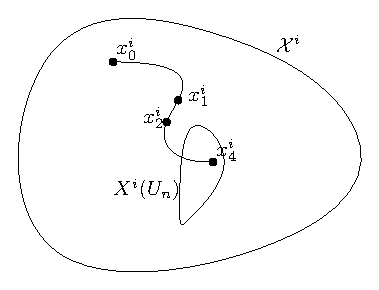
\includegraphics[width=0.5\linewidth]{invariant_set}
\caption{The image of the invariant set $\Xuinv$ after applying the control sequence $\Pastuseq$ is $\Xunobs(\Pastuseq)$}
\end{figure}

% Here I am trying to explain why I have been choosing a smaller class of systems
Interesting case scenarios happen when the knowledge about $\Xunobs(\Pastuseq)$ is preferable to the actual measure of the state $\xunobs$.
If $\Xunobs(\Pastuseq)$ is unbounded it can results in smaller abstraction (it can possibly create an infinite number of successors).
We will therefore focus on systems that have bounded invariant sets $\Xuinv$.

From now we will use linear time invariant systems. We use them mainly for their ease of manipulation.